\documentclass[UTF8]{article}
\usepackage{graphicx}
\usepackage{subfigure}
\usepackage{amsmath}
\usepackage{makecell}
\usepackage[utf8]{inputenc}
\usepackage[space]{ctex} %中文包
\usepackage{listings} %放代码
\usepackage{xcolor} %代码着色宏包
\usepackage{CJK} %显示中文宏包
\usepackage{float}
\usepackage{makecell}
\usepackage{diagbox}
\usepackage{bm}
\usepackage{ulem} 
\usepackage{amssymb}
\usepackage{soul}
\usepackage{color}
\usepackage{geometry}
\usepackage{fancybox} %花里胡哨的盒子
\usepackage{xhfill} %填充包, 可画分割线 https://www.latexstudio.net/archives/8245
\usepackage{multicol} %多栏包
\usepackage{enumerate} %可以方便地自定义枚举标题
\usepackage{multirow} %表格中多行单元格合并
\usepackage{wasysym} %可以使用wasysym里的一堆奇奇怪怪的符号

\geometry{left = 2.5cm, right = 2.5cm, bottom = 2.5cm, top = 3cm}

\definecolor{mygreen}{rgb}{0,0.6,0}
\definecolor{mygray}{rgb}{0.5,0.5,0.5}
\definecolor{mymauve}{rgb}{0.58,0,0.82}

\lstset{
	backgroundcolor=\color{white}, 
	%\tiny < \scriptsize < \footnotesize < \small < \normalsize < \large < \Large < \LARGE < \huge < \Huge
	basicstyle = \scriptsize,       
	breakatwhitespace = false,        
	breaklines = true,                 
	captionpos = b,                    
	commentstyle = \color{mygreen}\bfseries,
	escapeinside=``,
	extendedchars = false,
	frame = shadowbox, 
	framerule=0.5pt,
	keepspaces=true,
	keywordstyle=\color{blue}\bfseries, % keyword style
	language = verilog,                     % the language of code
	otherkeywords={string}, 
	numbers=left, 
	numbersep=5pt,
	numberstyle=\tiny\color{mygray},
	rulecolor=\color{black},         
	showspaces=false,  
	showstringspaces=false, 
	showtabs=false,    
	stepnumber=1,         
	stringstyle=\color{mymauve},        % string literal style
	tabsize=4,          
	title=\lstname,
	texcl=true  
}

%\sum\nolimits_{j=1}^{M}   上下标位于求和符号的水平右端,
%\sum\limits_{j=1}^{M}   上下标位于求和符号的上下处,
%\sum_{j=1}^{M}  对上下标位置没有设定,会随公式所处环境自动调整。

%%%%%%%%%%%%%画图包%%%%%%%%%%%%%
\usepackage{tikz}
%%%%%%%%%%%%%画图背景包%%%%%%%%%%%%%
\usetikzlibrary{backgrounds}

%%%%%%%%%%%%%在tikz中画一个顶点%%%%%%%%%%%%%
%%%%%%%%%%%%%#1:node名称%%%%%%%%%%%%%
%%%%%%%%%%%%%#2:位置%%%%%%%%%%%%%
%%%%%%%%%%%%%#3:标签%%%%%%%%%%%%%
\newcommand{\newVertex}[3]{\node[circle, draw=black, line width=1pt, scale=0.8] (#1) at #2{#3}}
%%%%%%%%%%%%%在tikz中画一条边%%%%%%%%%%%%%
\newcommand{\newEdge}[2]{\draw [black,very thick](#1)--(#2)}
%%%%%%%%%%%%%在tikz中放一个标签%%%%%%%%%%%%%
%%%%%%%%%%%%%#1:名称%%%%%%%%%%%%%
%%%%%%%%%%%%%#2:位置%%%%%%%%%%%%%
%%%%%%%%%%%%%#3:标签内容%%%%%%%%%%%%%
\newcommand{\newLabel}[3]{\node[line width=1pt] (#1) at #2{#3}}

%%%%%%%%%%%%%强制跳过一行%%%%%%%%%%%%%
\newcommand{\jumpLine} {\hspace*{\fill} \par}
%%%%%%%%%%%%%关键点指令,可用itemise替代%%%%%%%%%%%%%
\newcommand{\average}[1]{\left\langle #1\right\rangle }
%%%%%%%%%%%%%表格内嵌套表格%%%%%%%%%%%%%

\newcommand{\keypoint}[2]{$\bullet$\textbf{#1}\quad#2\par}
%%%%%%%%%%%%%<T>平均值表示%%%%%%%%%%%%%
\newcommand{\tabincell}[2]{\begin{tabular}{@{}#1@{}}#2\end{tabular}}%放在导言区
%%%%%%%%%%%%%大黑点item头%%%%%%%%%%%%%
\newcommand{\itemblt}{\item[$\bullet$]}
%%%%%%%%%%%%%大圈item头%%%%%%%%%%%%%
\newcommand{\itemc}{\item[$\circ$]}
%%%%%%%%%%%%%大星星item头%%%%%%%%%%%%%
\newcommand{\itembs}{\item[$\bigstar$]}
%%%%%%%%%%%%%右▷item头%%%%%%%%%%%%%
\newcommand{\itemrhd}{\item[$\rhd$]}
%%%%%%%%%%%%%定义为%%%%%%%%%%%%%
\newcommand{\defas}{=_{df}}
%%%%%%%%%%%%%蕴含%%%%%%%%%%%%%
\newcommand{\imp}{\rightarrow}

%%%%%%%%%%%%%双线分割线%%%%%%%%%%%%%
\newcommand*{\doublerule}{\hrule width \hsize height 1pt \kern 0.5mm \hrule width \hsize height 2pt}
%%%%%%%%%%%%%双线中间可加东西的分割线%%%%%%%%%%%%%
\newcommand\doublerulefill{\leavevmode\leaders\vbox{\hrule width .1pt\kern1pt\hrule}\hfill\kern0pt }
%%%%%%%%%%%%%左大括号%%%%%%%%%%%%%
\newcommand{\leftbig}[1]{\left\{\begin{array}{l}#1\end{array}\right.}
%%%%%%%%%%%%%矩阵%%%%%%%%%%%%%
\newcommand{\mat}[2]{\left[\begin{array}{#1}#2\end{array}\right]}
%%%%%%%%%%%%%可换行圆角文本框%%%%%%%%%%%%%
\newcommand{\ovalboxn}[1]{\ovalbox{\tabincell{l}{#1}}}
%%%%%%%%%%%%%设置section的counter, 使从0开始%%%%%%%%%%%%%
\setcounter{section}{0}

\title{计算机组成原理实验 实验报告}
\date{}

\begin{document}
%%%%%%%%%%%%%科大报告封面%%%%%%%%%%%%%
\maketitle
\begin{figure}[H]
	\centering
	
\includegraphics[width=2.5in]{xiaohui.png}\vspace{0.5cm}\\
	\large{
		实验题目:Lab3 单周期CPU\\
		学生姓名:王章瀚\\
		学生学号:PB18111697\\
		完成日期:\today\\
	}\vspace{2cm}
	
	\large{计算机实验教学中心制\\2019年09月\\}
	\thispagestyle{empty}
	\clearpage  % 清除当页页码
\end{figure}
\newpage

\section{实验题目}
Lab3 单周期CPU

\section{实验目的}
\begin{enumerate}
	\item 理解计算机硬件的基本组成、结构和工作原理;
	\item 掌握数字系统的设计和调试方法;
	\item 熟练掌握数据通路和控制器的设计和描述方法。
\end{enumerate}

\section{实验平台}
Vivado

\section{实验过程}
实验过程主要分为单周期CPU的设计和DBU的设计. 下面分块讲解二者.
\subsection{单周期CPU}
\subsubsection{基本过程}
单周期CPU的部分中, ALU, 寄存器堆, 数据存储器, 指令存储器等结构单元都已经在前面的实验中完成, 这里可以直接调用, 因此不再赘述这几个元件的相关实现.\par
这里需要讲解的部分有: 数据通路, 状态转换, 控制单元及其他代码等.\par
\subsubsection{数据通路}
这里数据通路基本上按照老师的来完成的. 下图是老师给定的数据通路.\par
\begin{figure}[H]
	\centering
	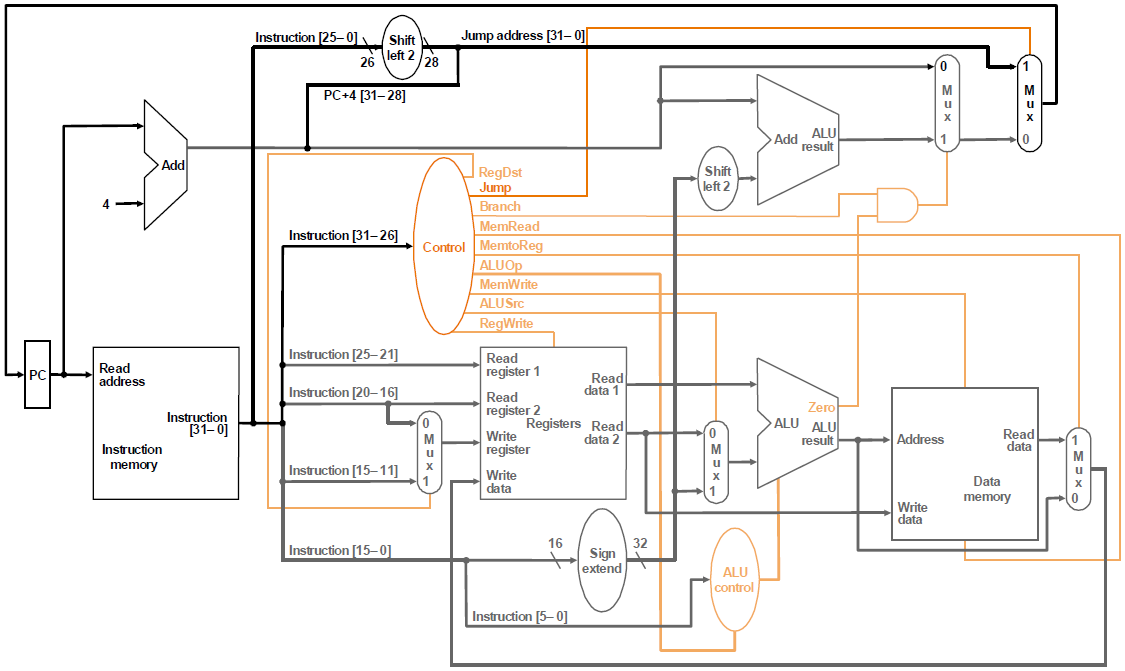
\includegraphics[width=\linewidth*2/3]{cpu_data_path_standard.png}
\end{figure}
而我对我完成的代码进行RTL分析, 能够得出下面的数据通路. 其中各个模块的功能已经在图中具体标识了.\par
\begin{figure}[H]
	\centering
	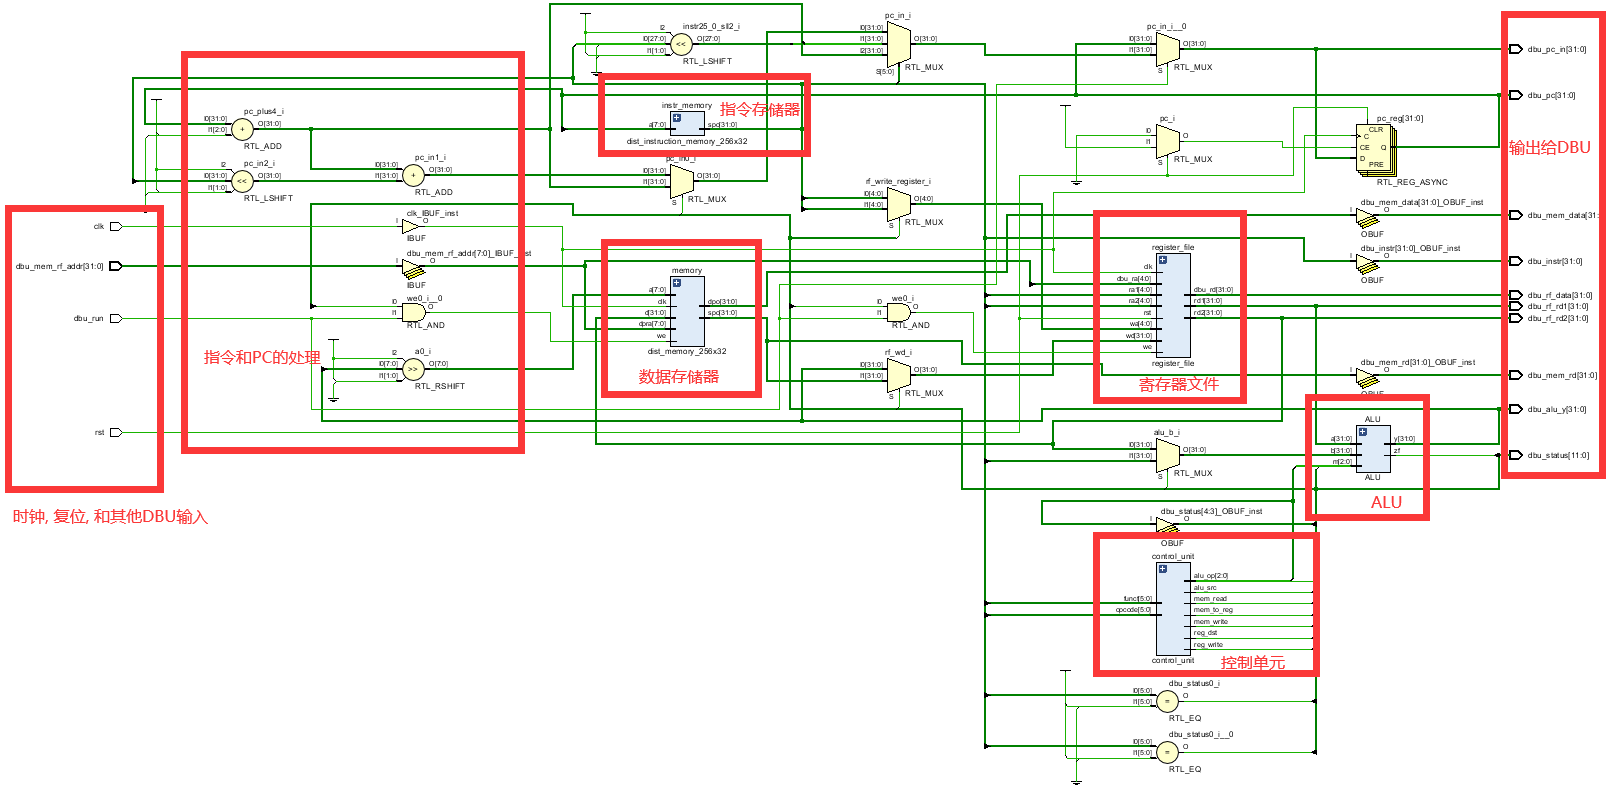
\includegraphics[width=\linewidth]{cpu_data_path_mine.png}
\end{figure}
\subsubsection{状态转换}
单周期的CPU状态机比较简单, 某种程度上可以认为状态只由PC决定. 因此它的状态转换图也比较简单. 如下.\par
\begin{figure}[H]
	\centering
	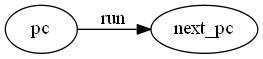
\includegraphics[width=\linewidth/5]{phase_diagram.png}
\end{figure}
\subsubsection{代码讲解}
\begin{enumerate}
	\item 数据通路代码\\
	这里只展示CPU内部的数据通路, 传出去给DBU的数据通路就是对应传递即可, 没有什么特别的地方.\\
	而CPU内部数据通路按照老师给出的数据通路进行连接, 其中值得注意的是, 由于存储器的地址应该为字地址, 传入地址的时候需要进行左移两位的操作. 代码如下:
	\begin{lstlisting}[language=verilog]
// 指令存储器
dist_instruction_memory_256x32 instr_memory(.a(pc[9:2]), .spo(instr));
// 指令存储器 - 寄存器文件
//// 选择写寄存器
assign rf_write_register = reg_dst == 1'b0 ? instr[20:16] : instr[15:11];
// 寄存器文件
register_file register_file(.clk(clk), .rst(rst),
                            .ra1(instr[25:21]), .rd1(rf_rd1),
                            .ra2(instr[20:16]), .rd2(rf_rd2),
                            .dbu_ra(dbu_mem_rf_addr[4:0]), .dbu_rd(dbu_rf_data),
                            .wa(rf_write_register), .we(reg_write & dbu_run), .wd(rf_wd));
// 寄存器文件 - ALU
//// 带符号扩展后十六位
assign instr_imm = {{16{instr[15]}}, instr[15:0]};
//// 选择alu\_src
assign alu_b = (alu_src == 1'b0) ? rf_rd2 : instr_imm;
// ALU
ALU ALU(.m(alu_op), .a(rf_rd1), .b(alu_b), .zf(alu_zero), .y(alu_y));
// ALU - 数据存储器
assign mem_addr = alu_y;
// 数据存储器
dist_memory_256x32 memory(.a(mem_addr >> 2), .d(rf_rd2), .dpra(dbu_mem_rf_addr), .clk(clk), .we(mem_write & dbu_run), .spo(mem_rd), .dpo(dbu_mem_data));
assign rf_wd = mem_to_reg == 1'b0 ? alu_y : mem_rd;
// 控制单元
control_unit control_unit(.opcode(opcode), .funct(funct), .reg_dst(reg_dst),
						  .reg_write(reg_write), .mem_read(mem_read),.mem_to_reg(mem_to_reg),
						  .mem_write(mem_write), .alu_op(alu_op), .alu_src(alu_src));
	\end{lstlisting}
	
	\item PC状态更新\\
	这一部分的代码使得PC状态能够进行状态转移.
	\begin{lstlisting}[language=verilog]
// PC的更新
wire [31:0] pc_plus4;
wire [27:0] instr25_0_sll2;
assign pc_plus4 = pc + 4;
assign instr25_0_sll2 = instr[25:0] << 2;
always @(*) begin
    if(dbu_run == 1'b0) begin
        pc_in = pc;
    end
    else begin
    	// 针对不同跳转指令作不同的PC处理
        case(opcode)
            BEQ_op: pc_in = alu_zero == 1'b1 ? pc + 4 + (instr_imm<<2) : pc + 4;
            J_op: pc_in = {pc_plus4[31:28], instr25_0_sll2[27:0]};
            default: pc_in = pc + 4;
        endcase
    end
end
always @(posedge clk, posedge rst) begin
    if(rst) begin
        pc <= 32'h0000_0000;
    end
    else begin
        pc = pc_in;
    end
end
	\end{lstlisting}
	
	\item 控制单元\\
	这部分是CPU的控制单元的代码. 它完成了对整个CPU各个地方的使能等信号的控制.\\
	这里主要就是针对每个指令进行解析, 判断各个指令需要使能哪些信号, 失能哪些信号. 代码如下.
	\begin{lstlisting}[language=verilog]
module control_unit
    #(
    parameter ADD_op = 6'b000000,
    parameter ADD_funct = 6'b100000,
    parameter ADDI_op = 6'b001000,
    parameter LW_op = 6'b100011,
    parameter SW_op = 6'b101011,
    parameter BEQ_op = 6'b000100,
    parameter J_op = 6'b000010,
    parameter ALU_ADD = 3'b000,
    parameter ALU_SUB = 3'b001,
    parameter ALU_AND = 3'b010,
    parameter ALU_OR = 3'b011,
    parameter ALU_XOR = 3'b100
    )
    (
    input [5:0] opcode,
    input [5:0] funct,
    output reg reg_dst, reg_write, mem_read, mem_to_reg, mem_write, alu_src,
    output reg [2:0] alu_op
    );
       
    // 控制单元
    always @(*) begin
        {reg_dst, reg_write, mem_read, mem_to_reg, mem_write, alu_op, alu_src} = 9'h0_0000_0000;
        case(opcode)
            ADD_op: begin
                case(funct)
                    ADD_funct: begin
                        reg_dst = 1'b1; reg_write = 1'b1; alu_op = ALU_ADD;
                    end
                    default: {reg_dst, reg_write, mem_read, mem_to_reg, mem_write, alu_op, alu_src} = 9'h0_0000_0000;
                endcase
            end 
            ADDI_op: begin
                alu_src = 1'b1; reg_write = 1'b1; alu_op = ALU_ADD;
            end
            LW_op: begin
                alu_src = 1'b1;
                mem_to_reg = 1'b1;
                reg_write = 1'b1;
                mem_read = 1'b1;
                alu_op = ALU_ADD;
            end
            SW_op: begin
                alu_src = 1'b1;
                mem_write = 1'b1;
                alu_op = ALU_ADD;
            end
            BEQ_op: alu_op = ALU_SUB;
            default: {reg_dst, reg_write, mem_read, mem_to_reg, mem_write, alu_op, alu_src} = 9'h0_0000_0000;
        endcase
    end
    
endmodule
	\end{lstlisting}
\end{enumerate}
至此, 单周期CPU的代码讲解部分结束.

\subsection{Debug Unit——DBU}
为了便于整个CPU的debug, 需要有一个DBU用以查看各个阶段中的各个输出, 寄存器和存储器的内容等, 以此进行便捷的debug工作.
\subsubsection{基本过程}
这个DBU单元主要有数码管显示控制, LED显示控制, 开关和电键输入解析等构成. 其中维护了一个地址寄存器, 用以查看寄存器文件和数据存储器的存储信息(这个寄存器内容的修改通过上按键和下按键调节).\par
由于没有FPGA开发板, 数码管的显示控制无法进行有效调试, 这里暂不讨论, 但为了证明有做这一项, 还是会把代码贴出.\par
除此之外, 就是一些数据的接线, 以及地址寄存器的内容修改, run信号的生成等. 下面将会讲解.
\subsubsection{数据通路}
DBU这一块的数据通路就由一些CPU模块, 取边沿模块和数码管模块之间的数据通路构成. 为了直观, 下面展示Vivado的RTL分析后的结果.\par
\begin{figure}[H]
	\centering
	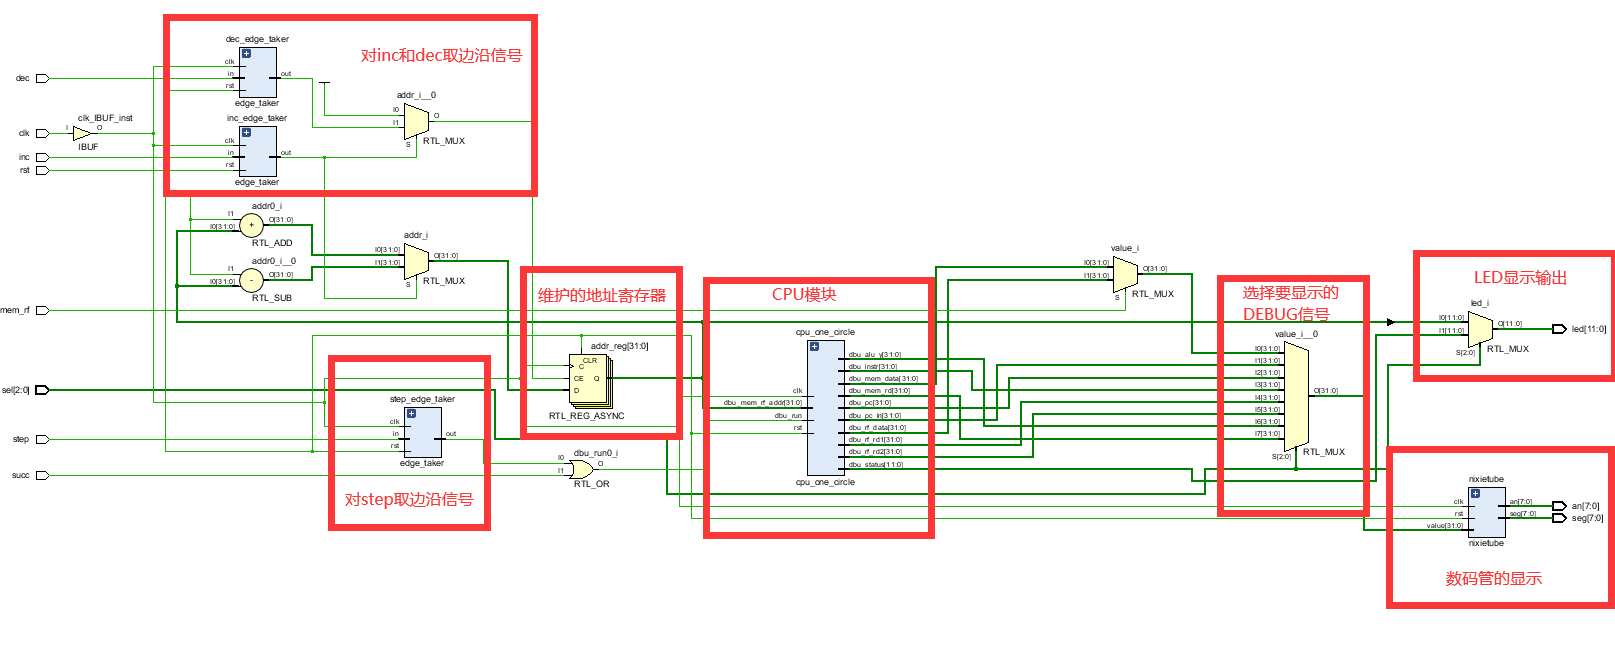
\includegraphics[width=\linewidth]{dbu_data_path.png}
\end{figure}
\subsubsection{状态转换}
DBU这块主要的状态就是选择地址的转换.
\begin{figure}[H]
	\centering
	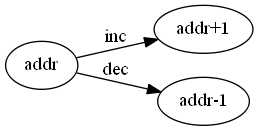
\includegraphics[width=\linewidth/5]{dbu_phase_diagram.png}
\end{figure}
\subsubsection{代码讲解}
\begin{enumerate}
	\item DBU数据通路
	\begin{lstlisting}[language=verilog]
// 取边沿信号(包括inc, dec和step的)
edge_taker #(.N(1)) inc_edge_taker(.clk(clk), .rst(rst), .in(inc), .out(inc_edge));
edge_taker #(.N(1)) dec_edge_taker(.clk(clk), .rst(rst), .in(dec), .out(dec_edge));
edge_taker #(.N(1)) step_edge_taker(.clk(clk), .rst(rst), .in(step), .out(dbu_run));
// CPU模块
cpu_one_circle cpu_one_circle(.clk(clk), .rst(rst), .dbu_run(dbu_run | succ),
                              .dbu_mem_rf_addr(dbu_mem_rf_addr), .dbu_rf_data(dbu_rf_data),
                              .dbu_mem_data(dbu_mem_data), .dbu_pc_in(dbu_pc_in),
                              .dbu_pc(dbu_pc), .dbu_instr(dbu_instr),
                              .dbu_rf_rd1(dbu_rf_rd1), .dbu_rf_rd2(dbu_rf_rd2),
                              .dbu_alu_y(dbu_alu_y), .dbu_mem_rd(dbu_mem_rd),
                              .dbu_status(dbu_status));
// 数码管模块
nixietube nixietube(.clk(clk), .rst(rst), .value(value), .an(an), .seg(seg));
// 传给数码管的要显示的值
always @(*) begin
    case(sel)
        3'b000: begin
            if(mem_rf) value = dbu_mem_data;
            else value = dbu_rf_data;
        end
        3'b001: value = dbu_pc_in;
        3'b010: value = dbu_pc;
        3'b011: value = dbu_instr;
        3'b100: value = dbu_rf_rd1;
        3'b101: value = dbu_rf_rd2;
        3'b110: value = dbu_alu_y;
        3'b111: value = dbu_mem_rd;
        default: value = 32'h0000_0000;
    endcase
end
	\end{lstlisting}
	
	\item 地址寄存器的increase和decrease\\
	根据前面数据通路取出的信号边沿, 进行inc和dec操作
	\begin{lstlisting}[language=verilog]
always @(posedge clk, posedge rst) begin
    if(rst) begin
        addr <= 4'b0000;
    end
    else begin
        if(inc_edge) addr <= addr + 1;
        else if(dec_edge) addr <= addr - 1;
    end
end
	\end{lstlisting}
	
	\item 数码管模块的实现\\
	这里直接用了上学期模拟与数字电路实验中完成的数码管, 虽然无从调试, 但应大体正确, 若拿到开发板可进行快速调试与修正.
	\begin{lstlisting}[language=verilog]

module nixietube(
    input clk,
    input rst,
    input [31:0] value,
    output reg [7:0] an,
    output reg [7:0] seg
    );
    
    // 分频计数器
    integer cnt_target_1000HZ;
    integer cnt_1000HZ;
    reg [3:0] digit;
    
    initial begin
        cnt_target_1000HZ = 10000;
        cnt_1000HZ = 0;
        an = 8'h00;
        seg = 8'h00;
    end
    
    always @(posedge clk, posedge rst) begin
        if(rst) begin
            cnt_1000HZ <= cnt_1000HZ + 1;
            an <= 8'b1111_1111;
            seg <= 8'h00;
            digit <= 4'b0000;
        end
        else begin
            if(cnt_1000HZ == cnt_target_1000HZ) begin
                cnt_1000HZ <=  0;
                case(an)
                    8'b1111_1110: begin an <= 8'b1111_1101; digit = value[3:0]; end
                    8'b1111_1101: begin an <= 8'b1111_1011; digit = value[7:3]; end
                    8'b1111_1011: begin an <= 8'b1111_0111; digit = value[11:7]; end
                    8'b1111_0111: begin an <= 8'b1110_1111; digit = value[15:11]; end
                    8'b1110_1111: begin an <= 8'b1101_1111; digit = value[19:15]; end
                    8'b1101_1111: begin an <= 8'b1011_1111; digit = value[23:19]; end
                    8'b1011_1111: begin an <= 8'b0111_1111; digit = value[27:23]; end
                    8'b0111_1111: begin an <= 8'b1111_1110; digit = value[31:27]; end
                    default: begin an <= 8'b1111_1111; digit = 4'b0000; end
                endcase
            end
            else begin
                cnt_1000HZ <= cnt_1000HZ + 1;
            end
        end
    end
    
    always @(*)
    begin
        case(digit)
            4'b0000: seg = 8'b1100_0000;
            4'b0001: seg = 8'b1111_1001;
            4'b0010: seg = 8'b1010_0100;
            4'b0011: seg = 8'b1011_0000;
            4'b0100: seg = 8'b1001_1001;
            4'b0101: seg = 8'b1001_0010;
            4'b0110: seg = 8'b1000_0010;
            4'b0111: seg = 8'b1111_1000;
            4'b1000: seg = 8'b1000_0000;
            4'b1001: seg = 8'b1001_0000;
            4'b1010: seg = 8'b1000_1000;
            4'b1011: seg = 8'b1000_0011;
            4'b1100: seg = 8'b1010_0111;
            4'b1101: seg = 8'b1010_0001;
            4'b1110: seg = 8'b1000_0110;
            4'b1111: seg = 8'b1000_1110;
        endcase
    end
endmodule
	\end{lstlisting}
\end{enumerate}

\section{实验结果}
实验结果部分同样分单周期CPU和DBU两块进行讲解. 但由于DBU完全包含CPU, 故这里不会对单周期CPU部分讲解太多. 若有疑问, 在DBU部分应该会有相应描述.\par
注意, 这里仿真所用的汇编代码为助教提供的代码, 这将极大地方便助教批阅!(见附件)\par
\subsection{单周期CPU}
因为后面的DBU仿真结果会按步骤详细讲解程序运行过程, 所以这一部分就展示一下整个仿真过程, 并且标识出PC和指令序列(结合汇编程序的beq跳转条件足以证明CPU工作正常), 和最后的程序正确运行时, 存储器的标识.\par
仿真结果如下图:\par
\begin{figure}[H]
	\centering
	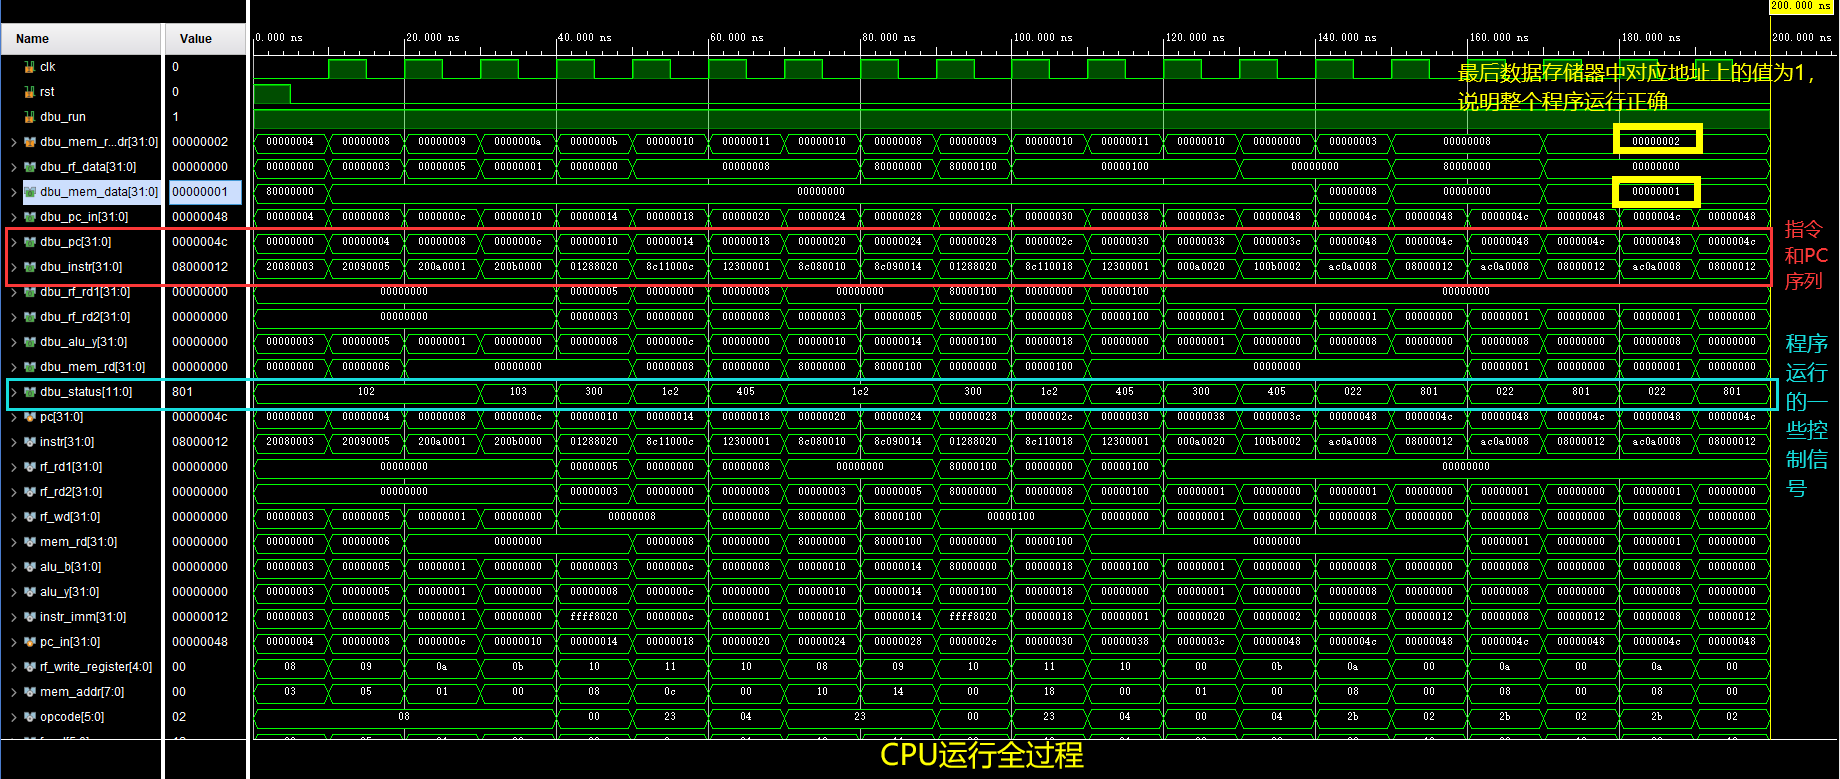
\includegraphics[width=\linewidth]{cpu.png}
\end{figure}
\subsection{Debug Unit——DBU}
这一部分的实验结果比较复杂, 按照助教对汇编代码分的几个部分来描述.
对于DBU\_LED的输出(仿真中变量为dbu\_status), 不再过分陈述, 因为只是进行数据传递, 如果这有错, 那么CPU将无法正常运行.\par
而寄存器文件和数据存储器的内容正确性, 也是程序运行到最后的\_success的必要条件, 因此仿真结果中会有显示, 但并不会做过多说明.\par
下面就用DBU分步讲解整个代码的运行过程!\par
\subsubsection{检查数据寄存器中的数据}
这一步用到了inc来检查数据寄存器中的数据, 这有两个好处:
\begin{enumerate}
	\item 可以检查inc等部分的正确性
	\item 可以检查数据存储器的工作是否正常
\end{enumerate}
仿真结果如下,
\begin{figure}[H]
	\centering
	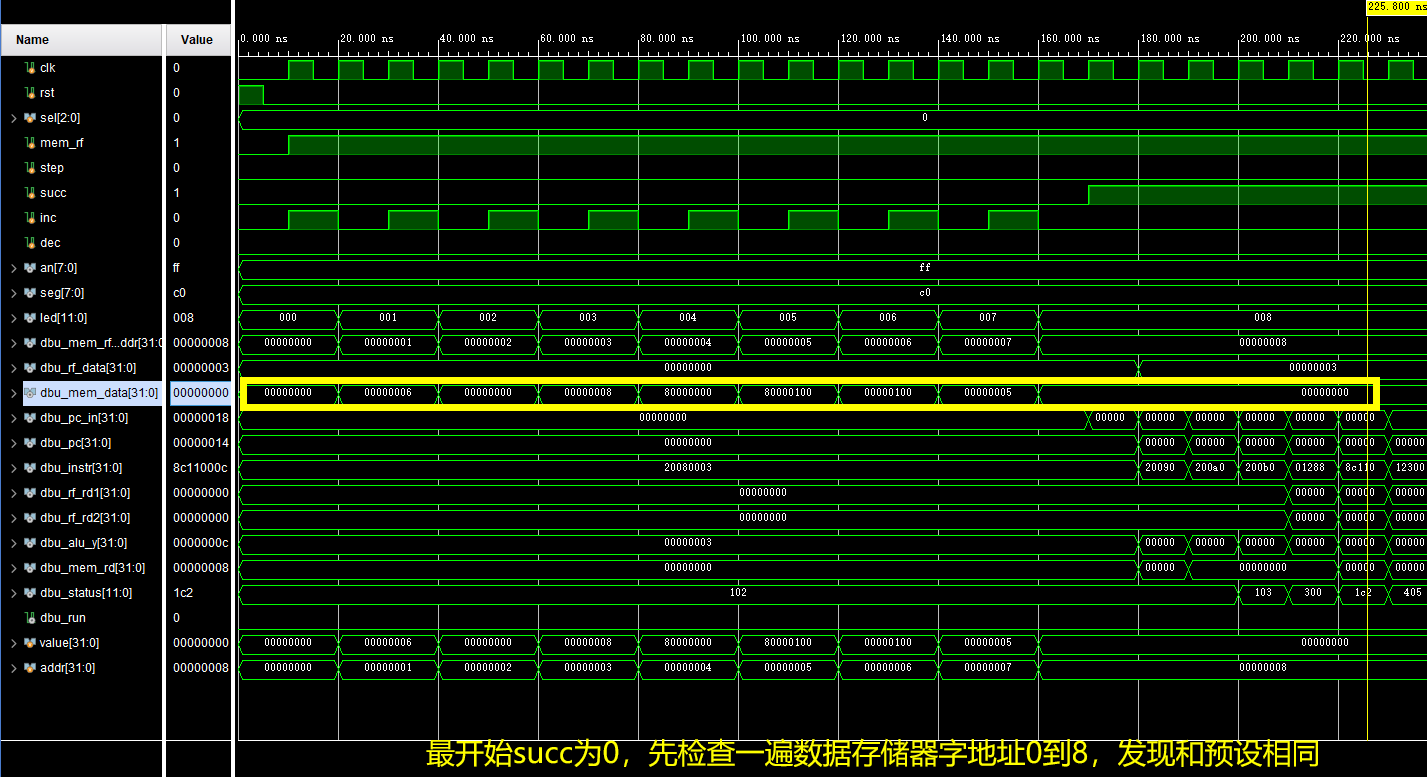
\includegraphics[width=\linewidth]{mem_data.png}
\end{figure}
\subsubsection{\_start部分}
\_start部分, 对几个寄存器做了addi等操作, 并做了一次lw, 而后beq. 如果能正常beq, 也可以说明代码运行正常.
仿真结果如下. 可以看到alu\_y的结果均正确, 并且pc\_in也表示将会进行程序正确运行时的跳转.
\begin{figure}[H]
	\centering
	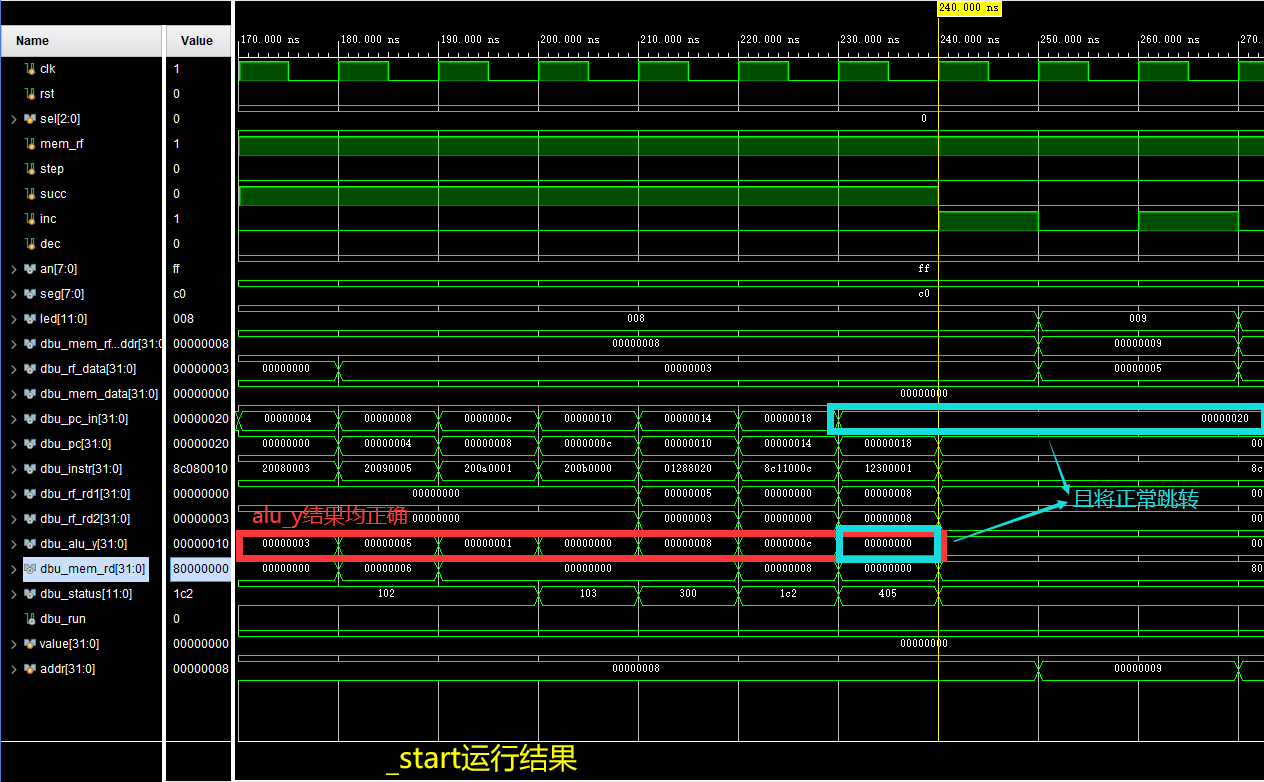
\includegraphics[width=\linewidth]{_start.png}
\end{figure}
这一步中, 也展示一下寄存器内容修改的正确性. 同时再次检验inc的可用性.
\begin{figure}[H]
	\centering
	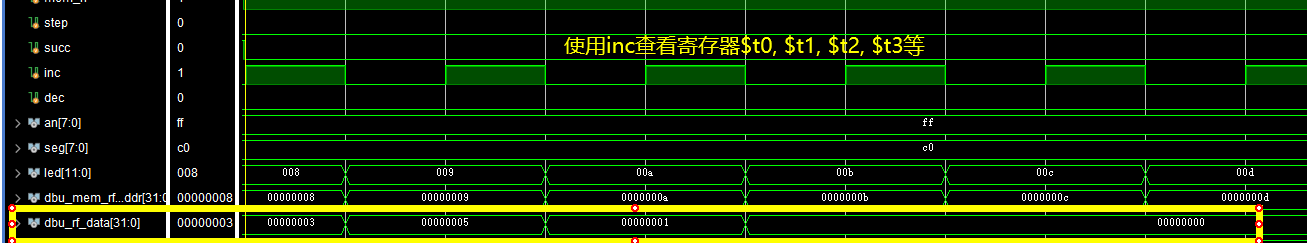
\includegraphics[width=\linewidth]{_start_data.png}
\end{figure}
\subsubsection{\_next1部分}
这一步进行了一些lw操作, 可以检查lw操作的正确处理, 并进行了beq. 同样, 如果能正常beq, 也可以说明代码运行正常.\par
同时, 为了检查step的可行性, 这一部分暂停使用succ, 改用step不断输入, 以逐条执行指令.
\begin{figure}[H]
	\centering
	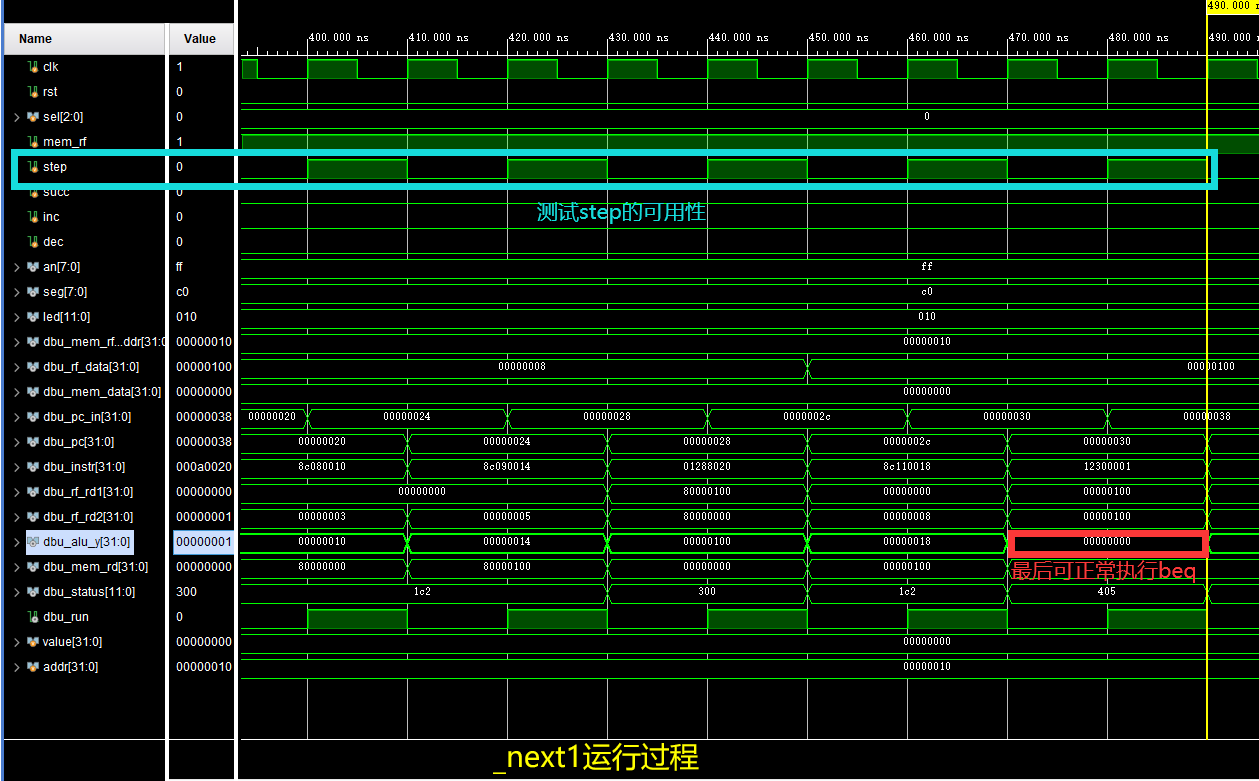
\includegraphics[width=\linewidth]{_next1.png}
\end{figure}
\subsubsection{\_next2和\_success部分}
这里主要是检查了寄存器\$0永远为0以及\_success部分的j指令.\par
并且最后展示一下数据存储器地址0x08(字地址为0x2)的数值为1, 表示整个程序运行是正确的.\par
下面展示了寄存器\$0永远为0, 因此能够正确地进行beq. 而在\_success阶段, 能够正常的jump(j指令), 仿真结果如下:
\begin{figure}[H]
	\centering
	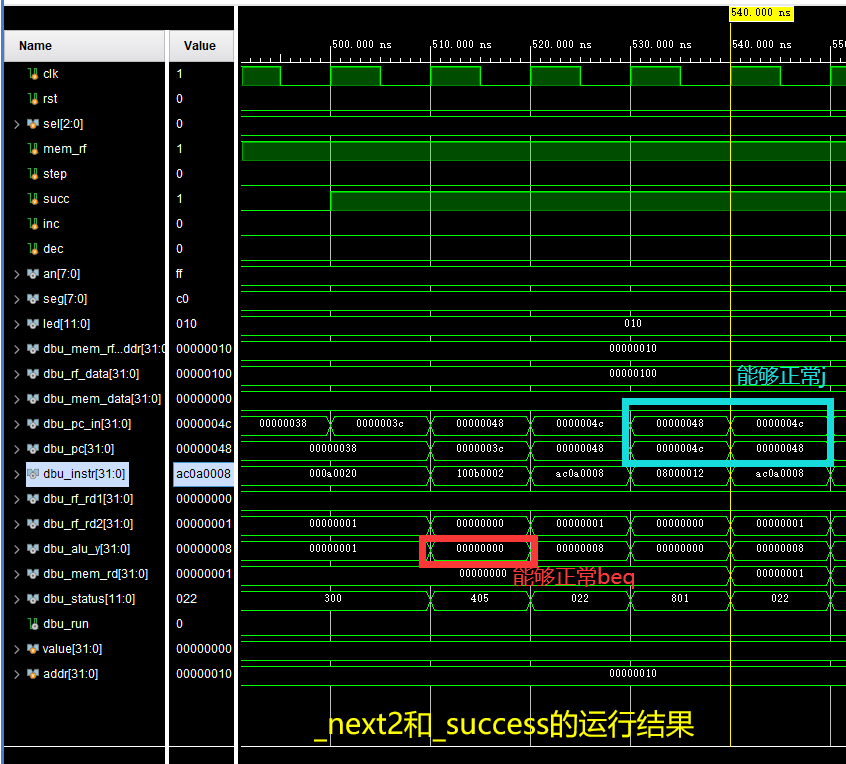
\includegraphics[width=\linewidth]{_next2_success.png}
\end{figure}
数据存储器地址0x08(字地址为0x2)的数值为1. 仿真结果如下图,
\begin{figure}[H]
	\centering
	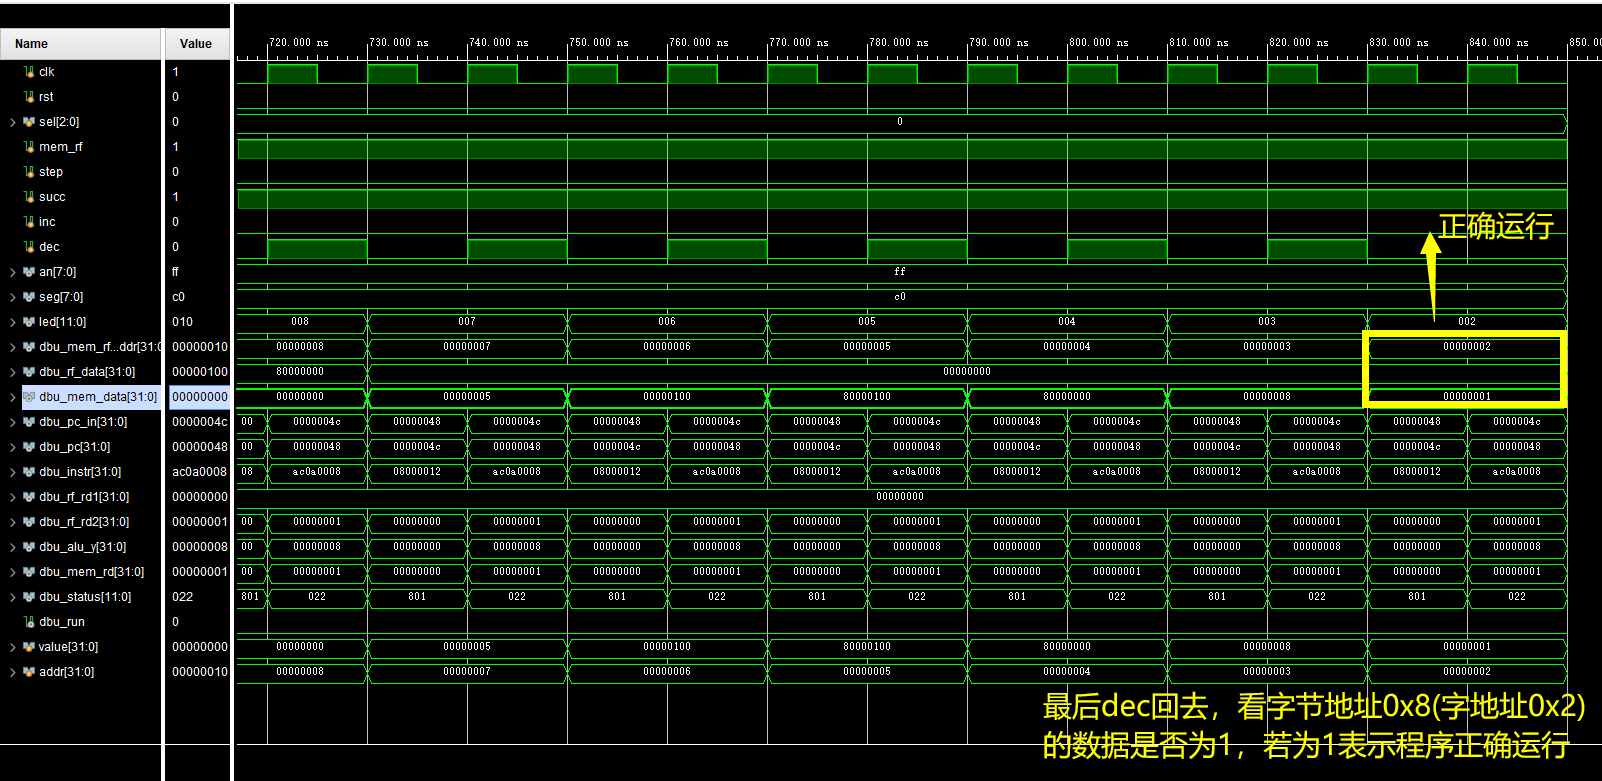
\includegraphics[width=\linewidth]{final_check.png}
\end{figure}
至此, DBU的仿真过程讲解完毕.

\section{思考题}
题目: 修改数据通路和控制器, 增加支持如下指令: \par
\begin{center}
	\ovalboxn{accm: rd $\leftarrow$ M(rs) + rt; 	op = 000000, funct = 101000}
\end{center}
这里需要修改的数据通路和控制器有如下:
\begin{enumerate}
	\item 控制单元 $\leftrightarrow$ 各个模块\\
	控制单元需要解析这条新的指令, 并且相应地去产生数据存储器, 寄存器文件等的存取使能信号.
	\item 寄存器堆rs $\leftrightarrow$ 数据存储器读地址
	需要将rs作为地址, 读出数据存储器上的M(rs)值.
	\item 数据存储器访存结果 $\leftrightarrow$ ALU
	将上述M(rs)结果传给ALU, 和rt进行加法运算
	\item ALU\_out $\leftrightarrow$ 寄存器堆写数据
	将上述ALU加法计算结果传给寄存器堆的写数据端口, 在下一个时钟上升沿进行写入.
\end{enumerate}
以上增加的数据通路和控制器足以完成这样一条指令.

\section{心得体会}
这是我第一次亲手完成一个CPU的verilog代码, 并附有DBU(Debug Unit), 虽然比较复杂, 但由于有了老师精细的讲解和各位助教的帮助, 整个过程比较顺利.\par
这次实验的收获主要是明白了单周期CPU设计原理, 并且对单周期CPU的了解更进一步. 此外, 还明白了怎么样去设计一个DBU来对自己设计的CPU进行检验.\par
虽然没能拿到FPGA开发板进行测试, 但仿真成功的结果属实令人开心!\par

\section{意见建议}
这次老师和助教们都准备得很充分, 没有什么太多建议.\par

\section{附件}
\begin{figure}[H]
	\centering
	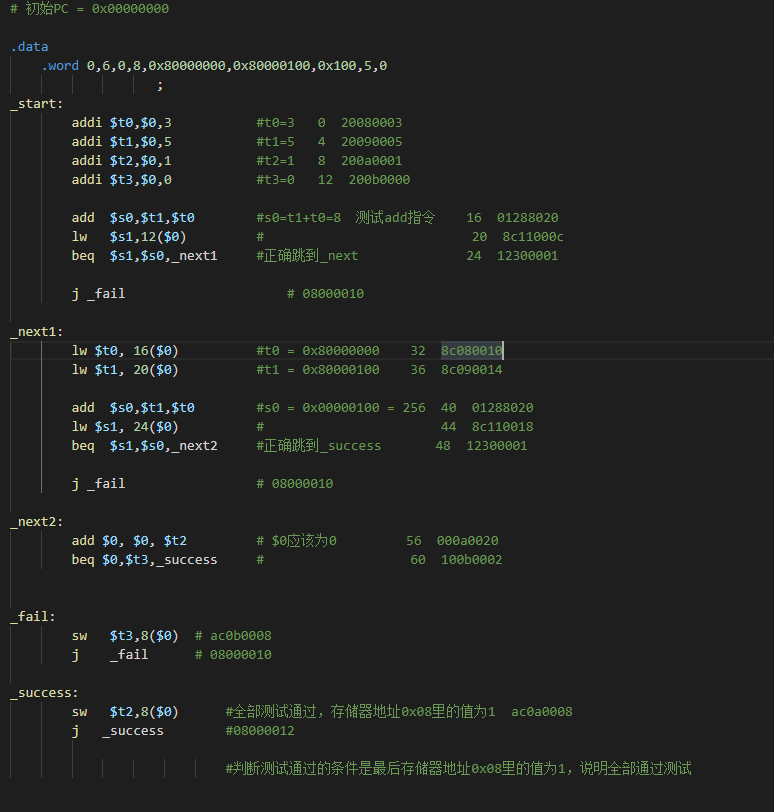
\includegraphics[width=\linewidth]{sim_asm.png}
\end{figure}


\end{document}






